\documentclass{article}
\usepackage[superscript,biblabel]{cite}
\usepackage{graphicx}

\graphicspath{{../../analysis/images/}}
\bibliographystyle{plain}

\title{Epistasis is widespread in the genetic control of transcription in humans}


\begin{document}

\maketitle


\begin{abstract}
A long standing question in human genetics is the extent to which epistasis, the phenomenon whereby one mutation's effect on a trait depends on other mutations present in the genome, contributes to complex traits. Though epistasis is known to arise from artificial gene manipulation studies in model organisms, and occasional examples have been shown in other species, few convincing examples exist for epistasis amongst natural polymorphisms in human traits. Its absence from empirical findings may simply be due to its unimportance in the genetic control of complex traits, but we hypothesised that it has previously been too technically difficult to detect due to statistical power and computational issues. Here we show that, using advanced computation techniques and a gene expression study design where any effects are expected to be large, evidence for abundant epistasis is found. In a cohort of 842 individuals with data on 7339 gene expression levels in whole blood, we found that after stringent correction for multiple testing the expression of 249 genes is controlled by 549 significant pairwise epistatic interactions. We attempted replication in two independent datasets and 421 show evidence of significance in at least one dataset. Several genes are controlled by multi-locus epistatic interactions whereby one cis-acting single nucleotide polymorphism (SNP) is modulated by several trans-acting SNPs. For example MBNL1 is controlled by an additive effect at rs13069559 which itself is controlled by trans-SNPs on 18 different chromosomes, with nearly identical genotype-phenotype (GP) maps for each cis-trans interaction. This study presents the first strong evidence for the widespread existence of epistasis emerging from natural genetic variation in humans.
\end{abstract}


\section{Main}

\subsection{Introduction}
The past decade has seen a tremendous amount of activity in mapping genetic polymorphisms that underlie complex traits. Typically, SNPs are treated as contributing linearly, independently, and cumulatively to the mean of a trait and this has been successful in identifying hundreds of causal variants. Yet outside the prism of association studies there is widespread evidence for epistasis, not only at the molecular scale in artificial double gene knockouts in experimental organisms but also at the evolutionary scale in fitness adaptation and speciation. Though its importance is frequently the subject of debate so far there is little convincing empirical evidence for epistasis playing a substantial role in the architecture of complex traits.

The detection of epistasis is hampered by power issues for several reasons, including increased dependence on linkage disequilibrium (LD) between causal SNPs and observed SNPs, increased model complexity in fitting interaction terms, and more extreme significance thresholds to account for increased multiple testing \cite{Hemani2013}. When genetic effect sizes are small, as is expected in most complex traits of interest, the power to detect epistasis diminishes rapidly. There are two ways to overcome this problem, either use extremely large sample sizes, or use traits that are likely to have large effect sizes. Because our focus was to ascertain the extent to which epistasis exists amongst natural genetic variation we opted for the latter approach and searched for epistasis controlling gene expression levels. Though they number in the thousands, these traits are typically heritable but much less polygenic, thus it is expected that any genetic effects will be relatively large, maximising the chance at detecting epistasis should it exist.


\subsection{Results}

\subsubsection{Initial search}
We searched for pairwise epistasis exhaustively in the BSGS dataset which comprises 842 individuals who are genotyped at 528,509 SNPs and who have gene expression levels measured in whole blood samples for 7339 genes. Recent hardware and software advances made it possible to perform the $1.03 \times 10^{15}$ statistical tests to complete this analysis. We used permutation analysis to calculate an experiment-wide significance threshold of $2.91 \times 10^{-16}$ at the 5\% family-wise error rate (Methods). SNP pairs were modelled for full genetic effects, including marginal additive and dominance at both SNPs plus four interaction terms. Though we could have used a less complex model to improve statistical efficiency, we deemed it important to be agnostic about the type of epistasis that might exist, and therefore chose not to over-parameterise the test. Because there are many large marginal effects present in these data it was necessary to perform several filtering steps to exclude SNP pairs that were significant due to marginal effects alone. All SNP pairs with LD $r^2 > 0.1$ were removed, and were required to have at least 5 data points in all nine genotype classes. If multiple SNP pairs were present on the same chromosomes for a particular expression trait then only the sentinal SNP pair was retained. Finally, a nested test contrasting the full genetic model against the marginal additive and dominance model was performed for each remaining SNP pair (Methods), resulting in 549 significant interactions after Bonferroni correction for multiple testing.

\subsubsection{Replication}
It is intrinsically difficult to replicate epistasis because the dependence on LD between observed SNPs and causal variants is on average four orders of magnitude higher than for independent additive effects. The significant SNP pairs were carried forward for replication in two independent datasets that used the same expression assays for analysing transcription in whole blood, Fehrmann ($n=1240$) and EGCUT ($n=891$). There was substantial evidence for overlap of interaction effects in all three datasets. Of the 480 original pairs that passed filtering in Fehrmann and EGCUT, 421 of the SNP pairs showed replication for the interaction test at the 5\% false discovery rate (FDR) level in at least one dataset, and 148 in both datasets (Supplementary Figure \ref{fig:qqplotfdr}). The congruence of the epistatic networks in both datasets is shown in Figure \ref{fig:fireworks}. We also report that 39 of the interactions from the discovery set were significant at the Bonferroni level in at least one replication set (Supplementary Figure \ref{fig:qqplotbonf}), and of these 18 were significant in both. The GP maps for these interactions are remarkably similar in all three datasets (Figure \ref{fig:gpmaps}), lending strong evidence for the veracity of these signals. We also attempted replication in the CHDWB dataset, but only 185 of the SNP pairs passed filtering because the sample size was small ($n=139$), and due to insufficient power there was no evidence for replication.


\subsubsection{Patterns of epistasis}



\subsubsection{Characterisation of genetic variation}



\subsubsection{Functional annotation}




\section{Notes}

Results


- Hundreds of significant pairwise interactions controlling gene expression replicate in two independent studies



- The genotype-phenotype maps for the most significant replications are consistent in all three datasets



- The proportion of the variance that is due to interactions is generally smaller than additive. There is an ascertainment bias in that there are no genetic interactions strong enough to be detected on their own, and large additive effects are required to push them above the threshold



- There are several examples of gene expression being controlled by a cis-SNP which in turn is modulated by multiple trans-SNPs. The effects are consistent 



- Functional annotation shows that proteins are not being changed at the codon level
- There is strong enrichment for enhancers
- There is tissue specific transcription regulation for cis SNPs - these are regulatory
- Trans SNPs are not found in tissue specific transcription regions.
- General enrichment for regulatory motif modifications
- Names of specific factors that are enriched.



- No explicit mechanism arises from looking at GP maps



- Chromosome interactions?



\clearpage
\section{Methods summary}




\clearpage
\section{Figure legends}

\begin{figure}
	\caption{\textbf{Replication of epistatic networks in two cohorts} Panel A shows the overall network of genetic interactions (edges) for each probe (red nodes) and their controlling SNPs (black nodes) from the discovery set. Panel B shows those interactions that were present at the 5\% FDR level in at least one replication dataset, and panel C shows which interactions were significant in both replication datasets.}
	\label{fig:fireworks}
\end{figure}

\begin{figure}
	\caption{\textbf{Replication of genotype-phenotype maps in 2 cohorts} The GP maps for each epistatic interaction that is significant at the Bonferroni level in both replication datasets. Each tile represents the expression level for that SNP-SNP genotype class. Phenotypes for each interaction within each cohort are scaled to be between 0 and 1.}
	\label{fig:gpmaps}
\end{figure}

\begin{figure}
	\caption{\textbf{Comparison of genetic variances} Panel A shows the proportion of phenotypic variation that is captured by additive, dominant and interaction components for all 529 significant interactions, ordered by total phenotypic variance explained by the SNP pair. Panel B shows the proportion of the genetic variance that is attributable to the three variance components, ordered by the proportion that is additive.}
	\label{fig:variancecomponents}
\end{figure}



\clearpage
\section*{}
\setcounter{figure}{0}

\begin{figure}
\centering
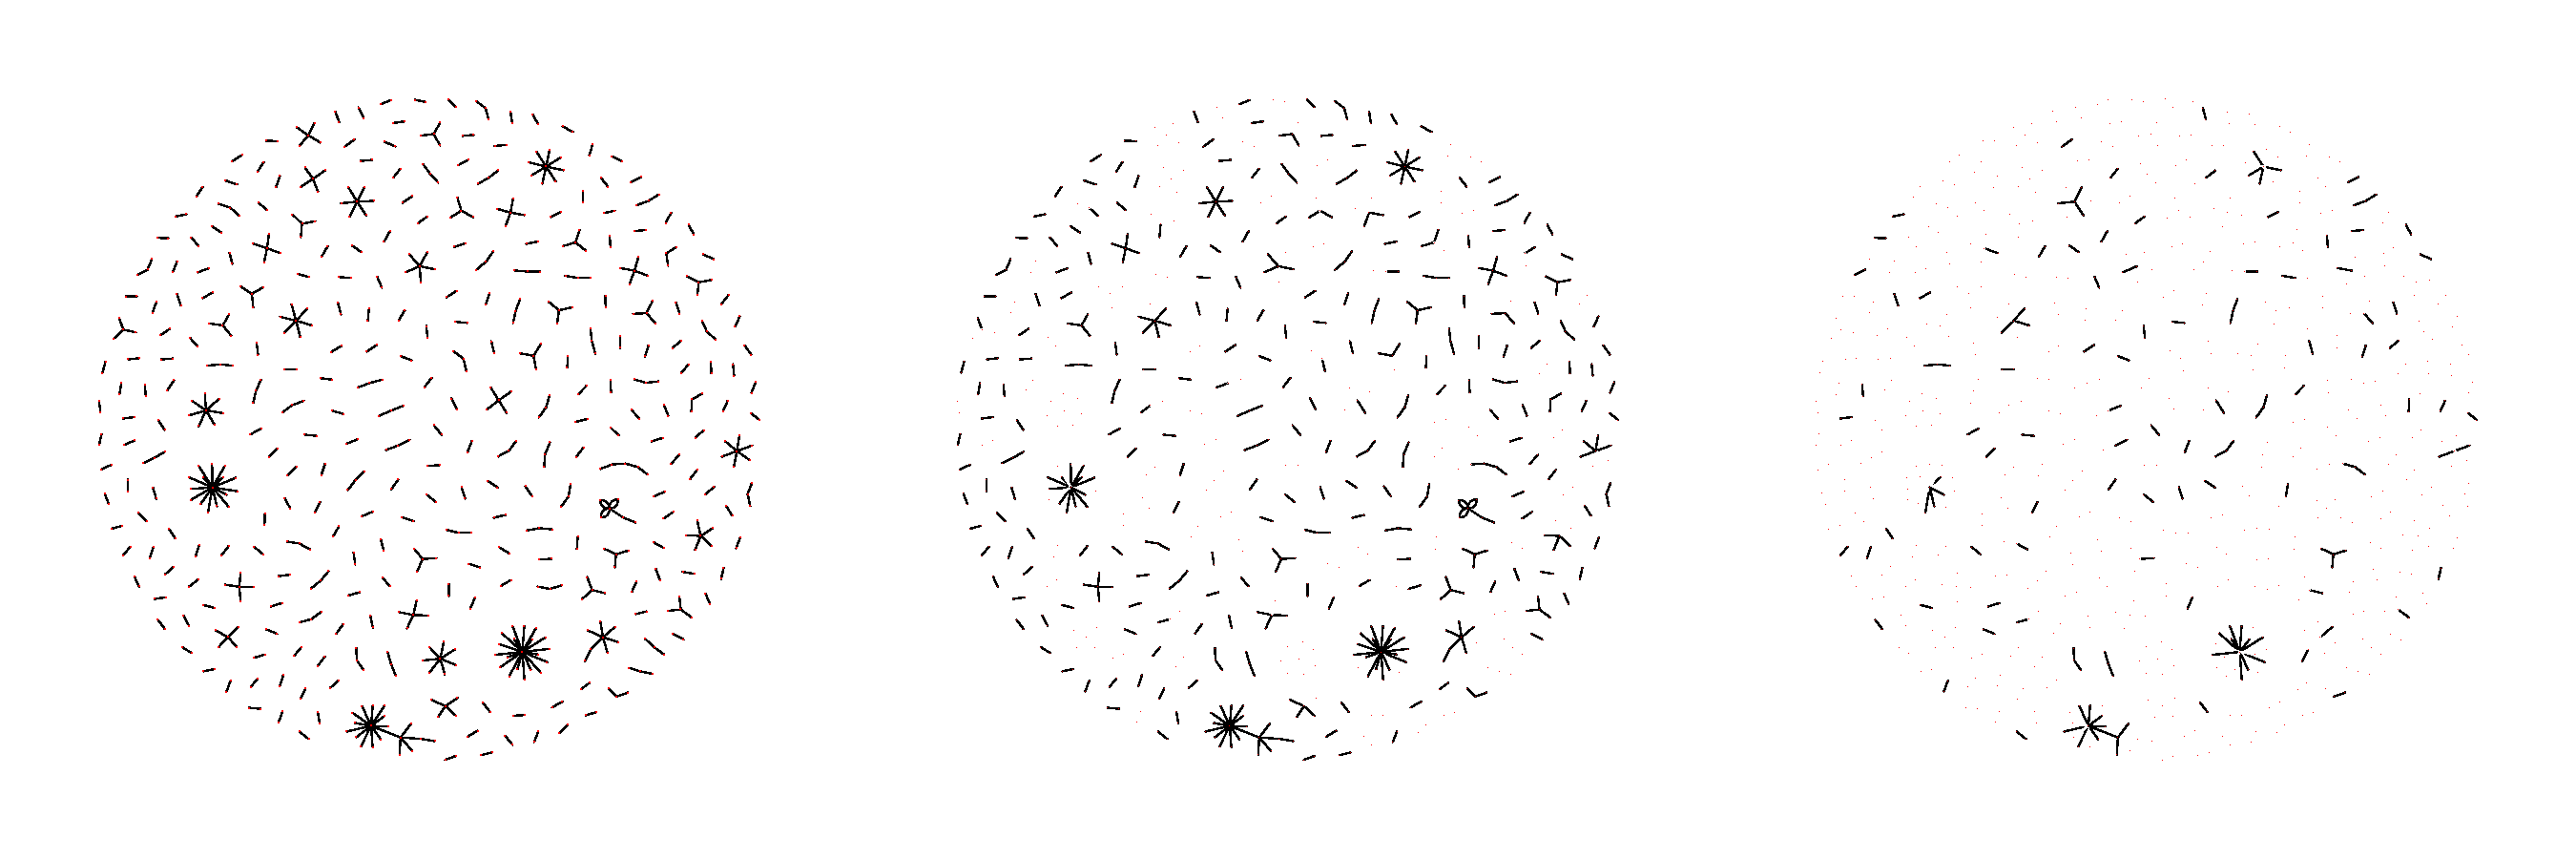
\includegraphics[width=5in]{hairballs_all_reps.pdf}
\caption{}
\end{figure}
\clearpage

\begin{figure}
\centering
\includegraphics[width=5in]{gpbonfrep.pdf}
\caption{}
\end{figure}
\clearpage

\begin{figure}
\centering
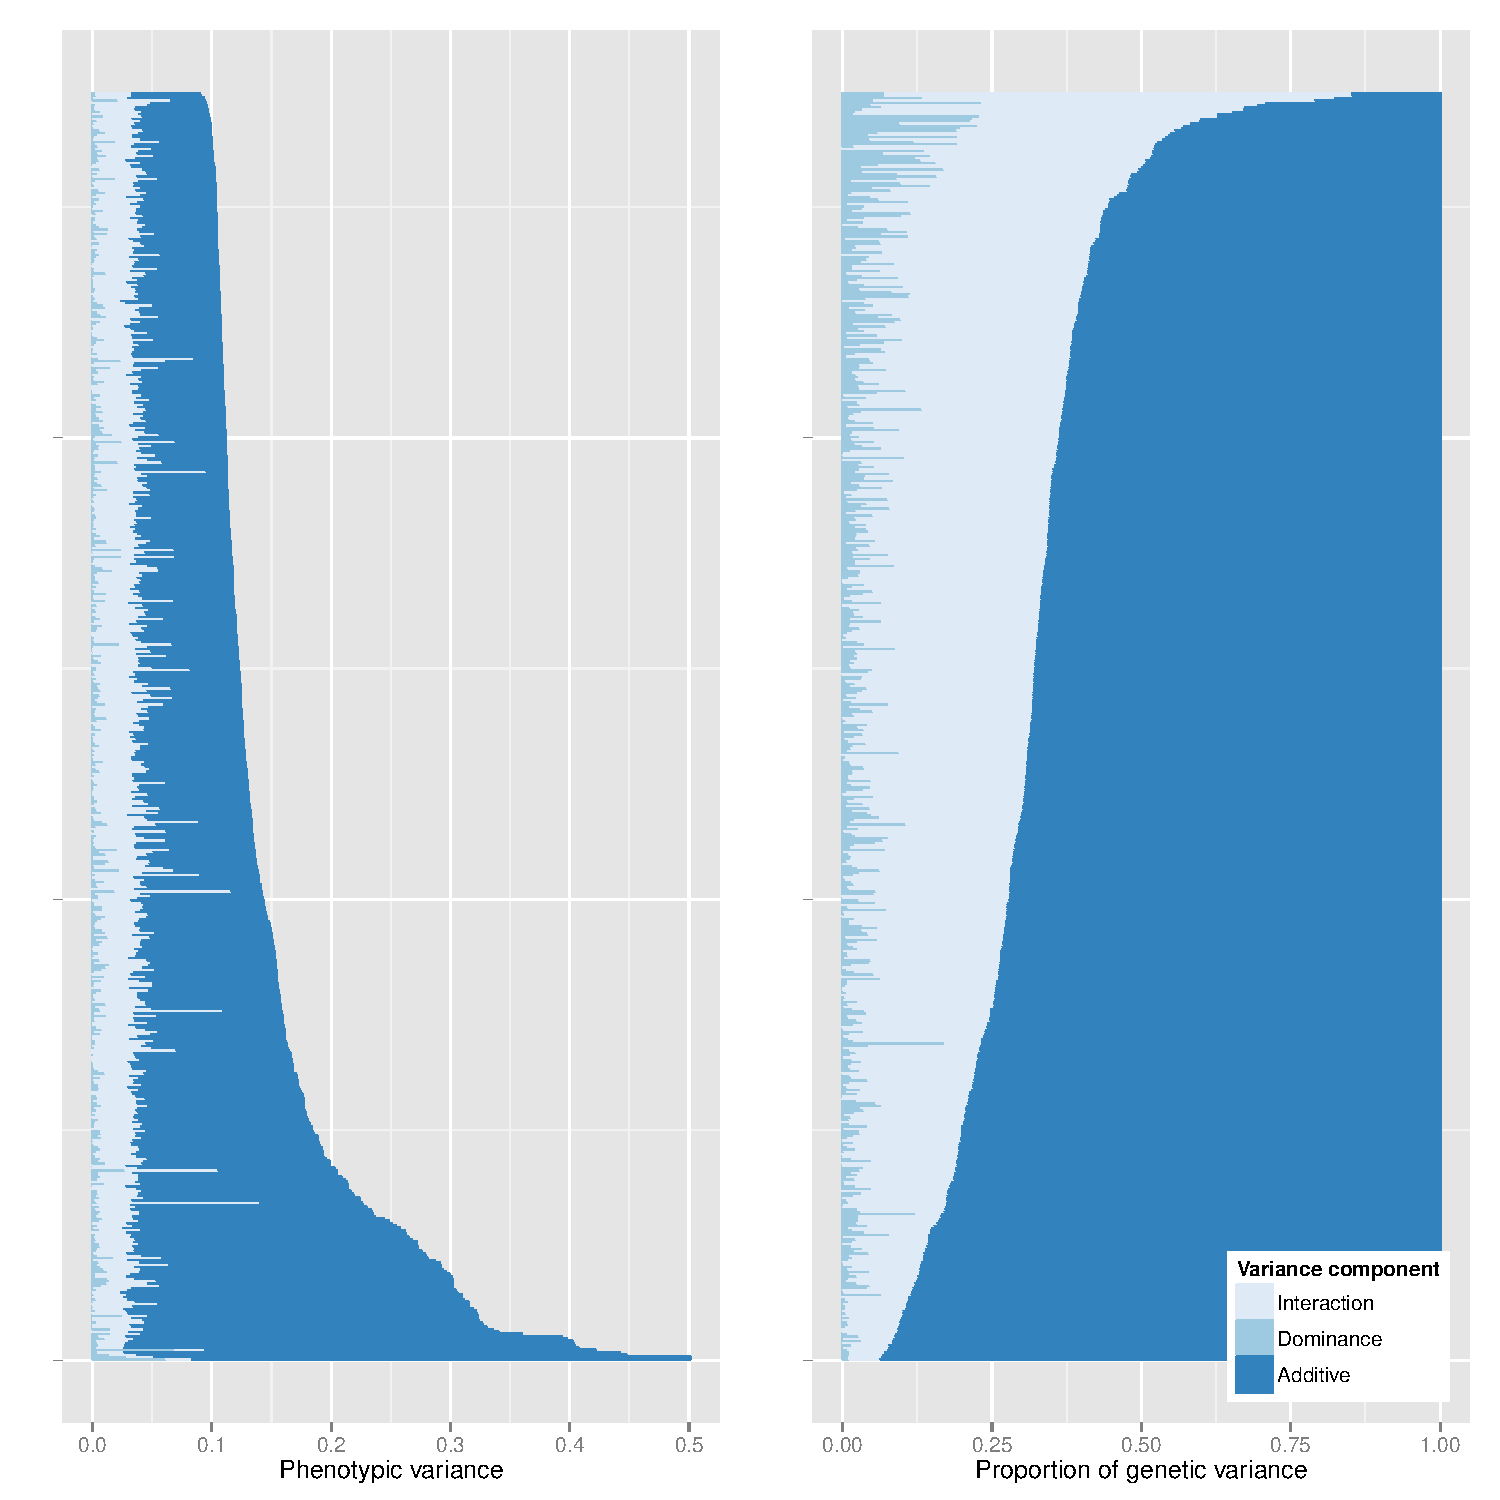
\includegraphics[width=5in]{variance_components.pdf}
\caption{}
\end{figure}
\clearpage

\section{Full Methods}

\subsection{Discovery data}

The Brisbane Systems Genetics Study (BSGS) comprises 862 Individuals of European descent from 274 independent families \cite{pmid22563384}. DNA samples from each individual were genotyped on the Illumina 610-Quad Beadchip by the Scientific Services Division at deCODE Genetics Iceland. Full details of genotyping procedures are given in Medland et al. \cite{Medland2009} Standard QC filters were applied and the remaining 528,509 SNPs were carried forward further analysis. 

Gene expression profiles were generated from whole blood collected with PAXgene TM tubes (QIAGEN, Valencia, CA) using Illumina HT12-v4.0 bead arrays. The Illumina HT-12 v4.0 chip contains 47,323 probes, although some probes are not assigned to RefSeq genes. We removed any probes that did not match the following criteria: contained a SNP within the probe sequence with MAF > 0.05 within 1000 genomes data; did not map to a listed ref-seq gene; were not significantly expressed (based on a detection $p$-value < 0.05) in 100\% of samples. After this stringent QC ~7000 [need to get exact number] probes remained for 2d-eqtl mapping. 

\subsection{normalisation}

Gene expression profiles were normalised and batch effects removed with the following procedures; Raw background expression were removed for each sample. Expression levels were then adjusted using Quantile and log2 transformation to standardise distribution between samples. To avoid inflation of the test statistic due to polygenic effects the following linear model was used to correct for batch and polygenic effects;  

\begin{equation}
y = \mu + c + p + s + a + g + e
\label{eq:lm}
\end{equation}
where $\mu$ is the population mean expression levels, $c$, $p$, $s$ and $a$ are vectors of chip, chip position, sex and generation respectively. $g$ is a random additive polygenic effect with a variance covariance matrix 


\begin{equation}
G_{ijk} = \left \{ 
\begin{array}{ll}
\sigma _a ^2 + \sigma _e ^2&        j = k \\ 
2\phi _{ijk} \sigma _a ^2& 			j \neq k \\
\end{array} \right.
\end{equation}

The parameters $\sigma _a ^a$ and $\sigma _e ^2$ are variance components for additive background genetic and environmental effects respectively. Here, we are using family based pedigree information rather than SNP based IDB to account for relationships between individuals and so $\phi _{ijk}$ is the kinship coefficient between individuals $j$ and $k$. The residual, $e$, from equation \ref{eq:lm} are assumed to follow a multivariate normal distribution with a mean of zero. These residuals are corrected for batch, sex, generation and polygenic effects. Residuals were standardised to Z-scores using a inverse-normal transformation and used as the adjusted phenotype for the pairwise epistasis scan. 

\subsection{exhaustive 2d-eQTL analysis}
We used epi-GPU software to perform an exhaustive scan for pairwise interactions, such that each SNP is tested against all other SNPs for statistical association with the expression values for each of the ~7000 probes. For each SNP-pair there are 9 possible genotype classes. We treat each genotype class as a fixed effect and fit an 8 d.f. $F$-test to test the following hypotheses:

\begin{equation}
H _0 : \sum _{i=1} ^3 \sum _{j=1} ^3 (\bar x _{ij} - \mu) ^2 = 0; 
\end{equation}

\begin{equation}
H _1 : \sum _{i=1} ^3 \sum _{j=1} ^3 (\bar x _{ij} - \mu) ^2 > 0; 
\label{eq:8df}
\end{equation}

where $\mu$ is the mean expression level and $x _{ij}$ is the pairwise genotype class mean for genotype $i$ at SNP 1 and genotype $j$ at locus B. This type of test does not parameterize for specific types of epistasis, rather it tests for the joint genetic effects at two loci. This has been demonstrated to be statistically more efficient when searching for a wide range of epistatic patterns (add refs), although will include any marginal effects of SNPs. \\[0.2cm]
 
The complete exhaustive scan for 7,000 probes comprises of $\sim$9.8$e^{14}$ $F$-tests. Due to the very large number of tests [plus nature of epistasis ....] we used a highly conservative series of filtering steps to identify study-wide significant epistasis associations to follow forward for replication analysis. Initially a significance threshold of $-log10$ 15.5. This threshold is the study-wide significance threshold determined by the number of independent tests for a 2D scan for a single probe / the number of probes analysed. This is likely to be conservative as this threshold assumes independence between probes. Following filtering on this threshold only SNP pairs with all 9 genotype classes and minimum genotype class size > 5 individuals were kept. We then calculated the linkage disequilibrium between SNPs in a pair and removed any pairs with $r^2$ > 0.1. We also removed any pairs containing SNPs for which single marker additive or dominance effects had been identified  in previous work (Powell et al. in Press). Sentinel  SNP pairs we retained from epistasis eQTL `peaks' comprising of multiple sets of pair-wise SNPs. At this stage $\sim$13,000 SNP pairs remained and were tested for the contribution of marginal and interaction terms by testing the 8d.f. \ref{eq:8df} verses a 4 d.f. model parameterizing for interaction terms only:

\begin{equation}
H _0: \sum _{i=1} ^3 \sum _{j=1} ^3 (\bar x _{ij} - \bar x _i - \bar x _j + \mu) ^2 = 0;
\end{equation}

\begin{equation}
H _1: \sum _{i=1} ^3 \sum _{j=1} ^3 (\bar x _{ij} - \bar x _i - \bar x _j + \mu) ^2 > 0;
\label{eq:4df}
\end{equation}

where $\bar x _i (\bar x _j)$ is the marginal class mean for genotype $i (j)$ at SNP A (B). Significance of interaction terms was determined using a bonferroni threshold of $0.05 / 13000 = 3.8e^{-6}$ 

We have attempted replication of the 2D scan significant results using three independent cohorts; Fehrmann, CHDWB and Rotterdam. Details of cohorts are as follows. \\[0.1cm]  

Fehrmann: $n$=1,469 \\[0.1cm]
The Fehrmann dataset consists of whole peripheral blood samples of 1,469 unrelated individuals from the United Kingdom and the Netherlands. Some of these individuals are patients, while others are healthy controls. Individuals were genotyped using Illumina HumanHap300, HumanHap370 or the 610 Quad platform. RNA levels were quantified using both the Illumina H8v2 platform (N = 229) and the HT12v3 platform (N = 1,240). \\[0.1cm]

CDHWB: $n$=189 \\ [0.1cm]
The Center for Health Discovery and Well Being (CDHWB) Study is a population based cohort consisting of 189 individuals collected in Atlanta USA. Gene expression profiles were generated with Illumina HT-12 V3.0 arrays from whole blood collected from Tempus tubes that preserve RNA. Whole genome genotypes were measured using Illumina OmniQuad arrays. \\[0.1cm]

Rotterdam: $n$=762 \\[0.1cm]
The Rotterdam Study is a large population based cohort collected to investigate the prevalence, incidence, and risk factors of chronic diseases among  Caucasians aged 45 years and over. Participants were genotyped using the Illumina 610K quad arrays. Whole blood of 768 samples was collected (PAXgene)and RNA hybridized to the Illumina Human HT-12v4 chips.



\clearpage
\section{References}
\bibliography{refs}


\clearpage
\section{Supplementary Figures}
\makeatletter 
\renewcommand{\thefigure}{S\@arabic\c@figure} 

\begin{figure}
\caption{\textbf{Q-Q plots of interaction $p$-values in two independent datasets}}
\label{fig:qqplotbonf}
\end{figure}

\begin{figure}
\caption{\textbf{Q-Q plots of replicated interaction $p$-values excluding the 20 most extreme $p$-values}}
\label{fig:qqplotfdr}
\end{figure}



\end{document}